\chapterimage{uvdisinfectionhero.jpg} % Chapter heading image

\chapter{Disinfection}
\nopagebreak
\begin{table}[H]
\begin{tabular}{| m{1cm} | m{15cm} |}
\hline
\multicolumn{2}{|l|}{\textbf{Expected   Range of Knowledge for Water Properties and Sources}}                                                                          \\ \hline
\multicolumn{2}{|l|}{\textit{Water   Distribution System Operator License Exams}}                                                                                      \\ \hline
D1 & Ability to   measure total chlorine                                                  \\ \hline
D1 & Ability to monitor   and interpret chlorine residual                                 \\ \hline
D1 & Knowledge of causes   of chlorine demand                                             \\ \hline
D1 & Knowledge of contact   time                                                          \\ \hline
D1 & Knowledge of   dechlorination techniques                                             \\ \hline
D1 & Knowledge of the   purpose of disinfection                                           \\ \hline
D1 & Ability to apply   disinfectant                                                      \\ \hline
D1 & Knowledge of water   main disinfectant techniques                                    \\ \hline
D1 & Knowledge of well   disinfection techniques                                          \\ \hline
D2 & Ability to choose the   proper disinfectant technique                                \\ \hline
D2 & Ability to recognize   when breakpoint has been met                                  \\ \hline
D2 & Knowledge of   advantages/disadvantages of chloramination                            \\ \hline
D2 & Knowledge of   chloramine compounds                                                  \\ \hline
D2 & Knowledge of chlorine   analysis techniques                                          \\ \hline
D2 & Knowledge of   disinfectant types and characteristics                                \\ \hline
D2 & Knowledge of factors   affecting chlorine disinfection                               \\ \hline
D2 & Knowledge of the   causes of DBPs                                                    \\ \hline
D2 & Knowledge of the   chlorine curve                                                    \\ \hline
D2 & Knowledge of the   definition of breakpoint chlorination                             \\ \hline
D3 & Ability to calculate   CT                                                            \\ \hline
D3 & Ability to recognize   abnormal levels of DBPs in the water distribution system      \\ \hline
D3 & Knowledge of chlorine   chemistry                                                    \\ \hline
D3 & Knowledge of DBP   compounds                                                         \\ \hline
D3 & Knowledge of DBP   formation                                                         \\ \hline
D3 & Knowledge of DBP   reduction methods                                                 \\ \hline

\end{tabular}
\end{table}

\newpage



\begin{table}[H]
\begin{tabular}{| m{1cm} |m{15cm} |}
\hline
\multicolumn{2}{|l|}{\textbf{Expected   Range of Knowledge for Water Properties and Sources}}                                                                      \\ \hline
\multicolumn{2}{|l|}{\textit{Water   Treatment Operator License Exams}}                                                                  \\ \hline
T1 & Knowledge of   acceptable chlorine residual levels                                   \\ \hline
T1 & Knowledge of   breakpoint chlorination chemistry                                     \\ \hline
T1 & Knowledge of chlorine   chemistry                                                    \\ \hline
T1 & Knowledge of common   chlorine compounds used for disinfection                       \\ \hline
T1 & Knowledge of   disinfectant byproduct formation                                      \\ \hline
T1 & Knowledge of   disinfectant properties and uses                                      \\ \hline
\end{tabular}
\end{table}
\newpage

\section{Background}\index{Disinfection!Background}
\begin{itemize}
\item The primary goal of water treatment is to ensure that the water is safe to drink and does not contain any disease-causing microorganisms. 
\item Disinfection refers to an operation to inactivate the microorganisms in water that can cause an infection or disease. These organisms are collectively referred to as pathogens and include many species of bacteria, fungus, protozoa, worms, viruses, etc.
\item The processes prior to disinfection - sedimentation and filtration, remove a large percentage of bacteria and other microorganisms from the water by physical means.
\item Disinfection \index{Disinfection}is different from sterilization, which is the complete destruction of all organisms which is expensive and unnecessary.
\item Water disinfection can be sub-divided as:
\begin{enumerate}
\item Primary disinfection \index{Disinfection!Primary disinfection}:
\begin{itemize}
\item Kills or inactivates bacteria, viruses, and other potentially harmful organisms in drinking water.
\item Disinfection prevents infectious diseases such as typhoid fever, hepatitis, and
cholera
\item Some disinfectants are more effective than others at inactivating certain
potentially harmful organisms.
\item Disinfection processes vary from water utility to water utility based on their
needs and to meet EPA treatment requirements.
\end{itemize}
\item Secondary disinfection \index{Disinfection!Secondary disinfection}:
\begin{itemize}
\item Maintenance of a disinfectant residual that prevents regrowth of microorganisms in the water distribution system between treatment and consumer.
\item Secondary disinfection maintains water quality by killing potentially harmful
organisms such as those that cause Legionnaire’s disease that may get in water as it moves through pipes.
\item Monochloramine is commonly used as a secondary disinfectant.
\end{itemize}
\end{enumerate}
\item Elements of an "ideal" disinfectant
\begin{itemize}
\item It must act in a reasonable time.
\item It must act as temperature or pH changes.
\item It must be nontoxic.
\item No harmful byproducts.
\item It must not add unpleasant taste or odor.
\item It must be readily available.
\item It must be safe and easy to handle and apply.
\item It must be easy to determine the concentration of.
\item It must be able to provide residual protection.
\item Pathogenic organisms must be more sensitive to the disinfectant than are non-pathogens.
\item It must be capable of being applied continually.
\item Versatile:  effective against all types of pathogens.
\item Fast-acting:  effective within short contact times
\item Robust: effective in the presence of interfering materials including particulates, suspended solids and other organic and inorganic constituents
\item Handy: easy to handle, generate, and apply (nontoxic, soluble, non-flammable, non-explosive)
\item Compatible with various materials/surfaces in WTPs (pipes, equipment)
\item Economical
\end{itemize}
\item In addition to the desirable characteristics of a disinfectant listed above, the disinfectant chosen must be able to kill off or deactivate pathogenic microorganisms by one of several possible methods, including:
\begin{enumerate}
\item Damaging the cell wall
\item Altering the ability to pass food and waste through the cell membrane
\item Altering the cell protoplasm
\item Inhibiting the cells’ conversion of food to energy
\item Inhibiting reproduction
\end{enumerate}
\item Most chemical disinfectants being strong oxidizers, aid the water treatment process by providing other benefits which include:  \begin{itemize}
\item Taste and odor control
\item Oxidize iron and manganese
\item Limit nuisance growths - algae 
\item Reduce mudball formation in filter media
\item Limit anaerobic sludge conditions
\item Improving coagulation
\end{itemize}

\end{itemize}

\section{Chlorination}\index{Chlorination}
\begin{itemize}
\item Despite potential drawbacks, chlorine is the disinfectant of choice.
\item In general, chlorination is effective, relatively inexpensive, and provides effective levels of disinfectant residual for safe distribution. 
\item Chlorine can be applied as:
\begin{itemize}
\item As a gas - elemental chlorine, $\mathrm{Cl}_{2}$:\\
\item Liquid (sodium hypochlorite) 
\item Solid (calcium hypochlorite)\\
each of these forms has advantages and disadvantages.
\end{itemize}
\end{itemize}
\subsection{Chlorine properties}\index{Chlorine properties}
\begin{itemize}
\item Chlorine is a yellowish-green gas at room temperature and atmospheric pressure
\item Chlorine gas can be pressurized and cooled to its liquid form for making it easy to ship and store. 
\item When liquid chlorine is released, it quickly turns into a gas that stays close to the ground (being heavier than air) and spreads rapidly.
\item While it is not explosive or flammable, as a liquid or gas it can react violently with many substances 
\item Chlorine is only slightly soluble in water (0.3 to 0.7\% by weight.) 
\item It has a characteristic disagreeable and pungent odor, similar to chlorine-based laundry bleaches, and is detectable by smell at concentrations as low as 0.2 to 0.4 ppm
\item It is about two and a half times as heavy as air
\item One volume of liquid chlorine yields about 460 volumes of chlorine gas. 
\item Liquid chlorine is amber in color and is about one and a half times as heavy as water 
\item Chlorine is an irritant to the eyes, skin, mucous membranes, and the respiratory system 
\end{itemize}

\subsection{Chlorine storage and safety}\index{Chlorine storage and safety}
\begin{itemize}
	\item Chlorine gas is lethal at concentrations as low as $0.1 \%$ air by volume. In nonlethal concentrations, it irritates the eyes, nasal membranes, and respiratory tract.
	\item Typically for smaller plants chlorine gas is shipped in  pressurized steel cylinders - 150 lb or 2000 lb (ton cylinder) size.  Larger plants may get their chlorine supply in rail tank cars.  \index{Chlorine cylinder}
	\item The daily chlorine usage is typically established based upon the weighing of the chlorine containers.
	\item The withdrawal rates from a chlorine cylinder is based on the temperature of the liquid in the cylinder, and thus the pressure of the gas. 
	\item As chlorine gas is withdrawn from the cylinder, it absorbs the heat from the surroundings.
	\item For low withdrawal rates, heat will be able to be transferred from the surrounding air to the container in time so that there is no drop in temperature or pressure, 
	\item If the chlorine withdrawal is larger, the air will not be able to transfer the heat quickly enough and the temperature (and pressure) of the chlorine will drop, thus resulting in a lower feed rate. 
	\item If high enough and prolonged enough, this can even result in ice formation around the outside of the container, further decreasing the withdrawal rate. 
	\item The most effective way to increase withdrawal rate from a single container is to circulate the surrounding air with a fan. Again, never apply heat to the containers.
	\item The maximum withdrawal rate for 100 or 150-pound cylinders should be limited to 40 pounds per day per cylinder. The maximum withdrawal rate for one-ton containers should be limited to 400 pounds per day per cylinder.
	\item If chlorine gas escapes from a container or system, being heavier than air, it will seek the lowest level in the building or area
	\item Only trained staff with access to proper personal protection equipment (PPE) including self-contained breathing apparatus, should handle the chlorine cylinders and address chlorine leak issues 
	\item When a leak is suspected, it is recommended that ammonia vapors be used to find the source. When ammonia vapor using a rag or brush, is directed at a leak, a white cloud will form. To produce ammonia vapor, a plastic squeeze bottle containing about 5 \% ammonia, aqua ammonia (ammonium hydroxide solution) should be used. A weaker solution such as household ammonia may not be concentrated enough to detect minor leaks
	\item All safety equipment should be located outside of the chlorine room and be easily accessed by all personnel
	\item Small leaks around valve stems can usually be corrected by tightening the packing nut or closing the valve. A leak can also be reduced by removing the chlorine as rapidly as possible
	\item If it cannot be added to the process there are several chemicals which can be used to absorb the chlorine gas. For example, chlorine can be absorbed by using 1$\dfrac{1}{4}$ pounds of caustic soda or hydrated lime, or 3 pounds of soda ash per pound of chlorine. 
	\item If the leaking container can be moved, it should be transported to an outdoors area where minimal harm will occur. Keep the leaking part the most elevated so that gaseous chlorine will leak rather than liquid chlorine.
	\item If the leak is large, all persons in the adjacent area must be warned and evacuated. Only authorized persons equipped with the proper breathing apparatus, and protective measures to the eyes and body should investigate. 
	\item As water is not an efficient absorbent for chlorine and the fact that chlorine reacts with water to form very corrosive hydrochloric acid, never apply water to a leak or consider submerging a chlorine cylinder (for example, in a pond or tank), since it will probably float.
	\item Remember to keep windward of the leak.
	\item As chlorine cylinders pressure increases with temperature, as a safety measure the chlorine cylinders are fitted with fusible plug \index{Chlorine cylinder!Fusible plug} which melts between 158$^o$ and 165$^o$ F.
	\item Keep chlorine cylinder or container emergency repair kits available. Be familiar with their use and location.
	\item Leaks at fusible plugs and cylinder valves requires special handling and emergency equipment. The chlorine supplier must be notified immediately
	\item Pin hole leaks in cylinder walls or ton tanks can usually be stopped by mechanical pressure applications (clamps, turnbuckles, etc.). This only temporary and may require your ingenuity.
	\item Leaking containers cannot be shipped.
	\item In general, daily inspection of all chlorine cylinders will avoid major problems\\
	\item In order to respond to leaks in chlorine containers, kits specific to the size of the container have been developed by the Chlorine Institute \index{Chlorine storage and safety!Emergency kits}.
	\begin{itemize}
	\item Emergency Kit "A" is designed for use with the standard 100 and 150 pound capacity cylinders in chlorine service only. It contains devices and tools to contain leaks in and around the cylinder valve and in the side wall of chlorine cylinders.

\item Emergency Kit "B" is designed for use with the standard chlorine ton container. It contains devices and tools to contain leaks in and around the ton container valves and in the side wall of ton containers.

\item Emergency Kit "C" is designed for use with the standard chlorine tank car, chlorine cargo tank and portable tank in chlorine service.
	\end{itemize}
	
\end{itemize}

\subsection{Forms of chlorine}\index{Chlorination!Forms of chlorine}

\begin{itemize}
	\item Due to safety issues related to the use of chlorine gas, \textbf{hypochlorites} are often used in lieu of chlorine
	\item Types of hypochlorites
	\begin{itemize}
	\item Sodium hypochlorite (NaOCl) comes in a liquid form which contains up to 12.5\% chlorine \index{Chlorination!Forms of chlorine!Sodium hypochlorite (NaOCl)}
	\item Calcium hypochlorite (Ca(OCl)$_2$), also known as High-test Hypochlorite (HTH)\index{Chlorination!Forms of chlorine!Calcium hypochlorite or high-test hypochlorite (HTH)}, is a solid which is mixed with water to form a hypochlorite solution. Calcium hypochlorite is 65-70\% concentrated.
	\end{itemize}
	\item Hypochlorites decompose in strength over time while in storage. Temperature, light, and physical energy can all break down hypochlorites before they are able to react with pathogens in water. 

\end{itemize} 

\subsection{Chlorine reactions related to disinfection}\index{Chlorination!Chlorine reactions}


\textbf{Chlorine reacts with water to form hypochlorous and hydrochloric acids}\\
Cl$_2$ \hspace{0.8cm}	+ \hspace{0.3 cm}	 H$_2$O		\hspace{0.8cm} $\iff$ 
\hspace{0.8cm} HOCl	\hspace{0.8cm}	 +	\hspace{0.8cm}	 HCl \\
chlorine \hspace{0.8cm}	water \hspace{1.8cm}		 hypochlorous acid	\hspace{0.1cm}	 hydrochloric acid\\ 
	\vspace{0.5cm}
	\begin{itemize}
		\item Hypochlorous acid dissociates in water to form the hydrogen and hypochlorite ions\\
 HOCl \hspace{1.8 cm} $\iff$ \hspace{1.8 cm} H$^+$ \hspace{1.8cm} + 	\hspace{0.8cm}OCl$^-$\\ 
hypochlorous acid  \hspace{1.9 cm}      hydrogen ion   \hspace{1.5cm}           hypochlorite ion

		\begin{itemize}
			\item Hypochlorous acid is the most effective form of chlorine available to kill microorganisms
			\item Hypochlorite ions is much less efficient disinfectant
		\end{itemize}

		\item The concentration of hypochlorous acid and hypochlorite ions \index{Chlorination!Chlorine reactions!Hypochlorite ions} \index{Chlorination!Chlorine reactions!Hypochlorous acid}in chlorinated water will depend on the water's pH
		\begin{itemize}
			\item A higher pH facilitates the formation of more hypochlorite ions and results in less hypochlorous acid in the water
		\end{itemize}
		\item A significant percentage of the chlorine is still in the form of hypochlorous acid even between pH 8 and pH 9
		\end{itemize}


\subsection{Factors affecting chlorine disinfection}\index{Chlorination!Factors affecting disinfection}
The disinfection efficiency of chlorine depends on the following factors:\\
\begin{itemize}
	\item pH:  Disinfection is more efficient at a low pH when large quantities of hypochlorous acid are present than at a high pH when hypochlorite ions is the dominant species in the water
	\item Concentration:  Contact Time (CT) \index{Contact Time (CT)}:  For effective chlorine disinfection both sufficient chlorine dosages – concentration (C) as well as contact time (T) are necessary.   Generally both of these factors must be worked out experimentally for a given system
	\item Disinfection activity can be expressed as the product of disinfection concentration (C) and contact time (T) - CT
	\item The same CT values will achieve the same amount of inactivation
	\item Temperature:  Colder temperatures are less favorable for disinfection. 
Proper contacting or mixing or agitation:  This is necessary to make sure that the chlorine applied contacts or reaches the microbial cells
	\item Organic and inorganic material present:  The chlorine used by these organic and inorganic reducing substances including metal ions, organic matter and ammonia, is defined as the chlorine demand.  So that the amount of chlorine that has to be added to wastewater for different purposes will also vary.
\end{itemize}

\subsection{Chlorine application}\index{Chlorination!Chlorine application}
\begin{itemize}
\item Continuous chlorination of systems less than 75 gpm is by the use of a hypochlorinator \index{Chlorination!Chlorine application!Hypochlorinator}where a motor driven pump pulls the hypochlorite solution out of a holding chamber and pumps it into the water to be treated.  Where the pipe from the pump joins the pipe carrying the raw water, the Venturi effect creates a small vacuum and pulls the chlorine solution into the water.
\item For larger system, chlorinators \index{Chlorination!Chlorine application!Chlorinator}- devices which introduce chlorine gas to water using liquid chlorine supplied in steel cylinders are used.
\item In the commonly used Vacuum Chlorinator:
\begin{itemize}
\item Chlorine gas is pulled from the cylinder into the source water by a vacuum created by water flowing through the injector and creating a negative head. 
\item This negative head forces open the pressure regulating valve on the cylinder and allows chlorine gas to flow out of the cylinder and into the chlorinator.
\item Once the gas has entered the chlorinator, the chlorine feed rate is measured using an indicator known as a rotameter
\item Just beyond the rotameter, the chlorine gas flows past a regulating device (a V-notch plug or a valve) which is used to adjust the chlorine feed rate.
\end{itemize}
\begin{figure}[h]
\begin{center}
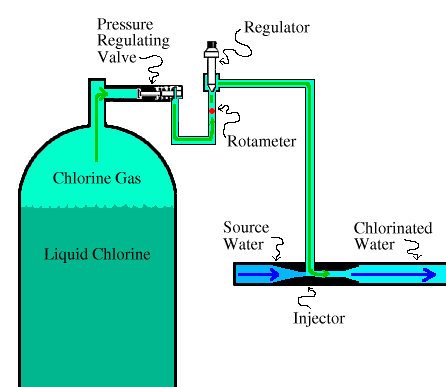
\includegraphics[scale=0.5]{VacuumChlorinator}\\
\captionof{figure}{Vacuum chlorinator}%\caption{}
\end{center}
\end{figure}
\end{itemize}
\vspace{-2em}
\subsection{Chlorination byproducts}\index{Chlorination!Byproducts}
\begin{itemize}
\item Main drawback of chlorine disinfection is the adverse health effects of the byproducts - Disinfection by-products (\colorbox{pink}{DBPs}) formed from its reaction with certain organic compounds present in the water.
\item  Adverse health effects on humans exposed to DBPs through drinking-water and oral, dermal, and inhalational contact with chlorinated water, include cancers of vital organs.
\item Halogenated trihalomethanes (\colorbox{pink}{THMs}) and haloacetic acids (\colorbox{pink}{HAAs}) are two major classes of disinfection byproducts (DBPs) commonly found in waters disinfected with chlorine. 
\item At the present time, about 90\% of U.S. water utilities use chlorine to disinfect water. Although chlorine has virtually eliminated the risks of waterborne disease such as typhoid fever, cholera, and dysentery, recent studies have shown risks associated with byproducts of chlorine — a reason why water utilities already have been looking at alternative methods for disinfecting water.
\item Approaches for reducing DBPs includes:
\begin{itemize}
\item Avoiding pre-chlorination where chlorine is added to the raw water before coagulation and filtration.
\item Removal of organics using Aeration or adsorption on activated carbon 
\item reevaluating the chlorine dosing to a level which will accomplish the same degree of disinfection with a lower chlorine dosage.
\item Another current approach is using alternative disinfection methods.
\end{itemize}
\end{itemize}

\subsection{Chloroamination}\index{Chloroamination}
			\begin{itemize}
			\item When chlorine is added to water containing ammonia, chlorine reacts with ammonia to form chloramines \index{Chloramines}.
			
\item Water utilities practice chloroamination - practice of utilizing the disinfectant properties of chloramines, by feeding chlorine to the water containing ammonia.
\item Chloramines are not as reactive as chlorine and are not as effective as chlorine as primary oxidizers.  However, chloramines decay rate is much slower than that for chlorine.
\item Chloramine is used as a secondary disinfectant to maintain a disinfectant residual throughout the distribution system so that drinking water remains safe as it travels from the treatment facility to the customer.
\item One-third of all public water systems in the United States use chloramine for residual disinfection.
			
			\item Chloramines are formed by the controlled addition of ammonia to chlorinated water form monochloramine (NH$_2$Cl), often in the recommended chlorine to ammonia ratio of 4.5:1 to prevent nitrification.\\
NH$_3$ + HOCl → NH$_2$Cl + H$_2$O
			
			
			\item Chlorine reacts with ammonia as follows:  When chlorine is added to water containing ammonia:
				\begin{enumerate}
					\item First the free chlorine in contact with ammonia forms monochloramine and water

					$NH_3 + HOCl   \rightarrow NH_2Cl (monochloramine) + H2O$\\
											\begin{itemize}
							\item Monochloramine has disinfection properties\\
							\item Dominates when Cl:N mass ratio is 0 to 5:1\\
							\end{itemize}
					\item Monochloramine reacts further with chlorine to give dichloramine and water\\
					$HOCl + NH_2Cl \rightarrow NHCl_2 + H_2O$\\
					Also, monochloramine auto decomposes into dichloramine\\
					$2NH_2Cl \rightarrow NHCl_2 + NH_3$
						\begin{itemize}
							\item Dichloramine is formed between 5:1 and 7:1 Cl:N mass ratio
							\item Dichloramine is a more effective disinfectant than monochloramine but their use may cause taste and odor problems. Thus the water industry only uses monochloramine as a disinfectant.
						\end{itemize}
						$NH_2Cl + HOCl  \rightarrow NHCl_2 (dichloramine)$\\
						at pH $>$ 7.5, monochloramine is the dominant chloramine species as pH decreases from 7.5, dichloramine becomes the dominant chloramine species increases in the chlorine to nitrogen dose ratio results in corresponding increases of nitrogen trichloride, but only when the pH is $<$ 7.4\\
					\item Formation of nitrogen trichloride from the reaction of chlorine and dichloramine does not typically occur as it is the favored product at low pH - $<$4\\
					$NHCl_2 + HOCl  \rightarrow NCl_3 (nitrogen trichloride)$\\
					\item Additional $free \enspace chlorine \enspace + chloramines \enspace \rightarrow H^+ + H2O + N_2$
				\end{enumerate}
				\item Chloramine levels up to 4 milligrams per liter (mg/L) or 4 parts per million (ppm) are considered safe in drinking water. At these levels, harmful health effects are unlikely to occur.				
				\item Chloramines have disinfection properties albeit much lower than free chlorine (~5\% of free available chlorine) but last much longer in the system than free chlorine. 
				\item Monochloramine is about 2,000 and 100,000 times less effective than free chlorine for the inactivation of E. Coli and rotaviruses, respectively.

\end{itemize}
\subsection{Advantages of chloramines}\index{Chloramines!Advantages}
\begin{itemize}
\item As chloramines do not tend to react with organic compounds, its use can reduce the formation of cancer-causing disinfection byproducts, such as the trihalomethanes and haloacetic acids and also result in fewer taste and odor complaints. 
\item Chloramine being more stable, its residual and thus its disinfectant benefit can persist for several days.
\item Chloramine dosing systems are relatively easy to install and operate. It also is among the less expensive disinfectant alternatives to chlorine.
\end{itemize}
\subsection{Disadvantages of chloramines}\index{Chloramines!Disadvantages}
\begin{itemize}
\item Poorest Disinfection
\item No taste and odor control or other aesthetic quality benefits.
\item Chloramine levels are more difficult to regulate than chlorine levels.  \item Microbes can nitrify \index{Nitrification} free ammonia remaining in the distribution system into nitrates (NO$_3^{\enspace-}$) and nitrite (NO$_2^{\enspace-}$). Nitrates interfere with the oxygen carrying capacity of the blood and is of great concern particularly to newborn babies and pregnant woman.
\end{itemize}			
	\subsection{Breakpoint chlorination}\index{Breakpoint chlorination}		
			Breakpoint chlorination curve provides a graphical representation of the fate of chlorine as it is being added to water containing ammonia and serves as an important tool for systems using chloramination, 
The breakpoint curve can be explained as follows:\\
			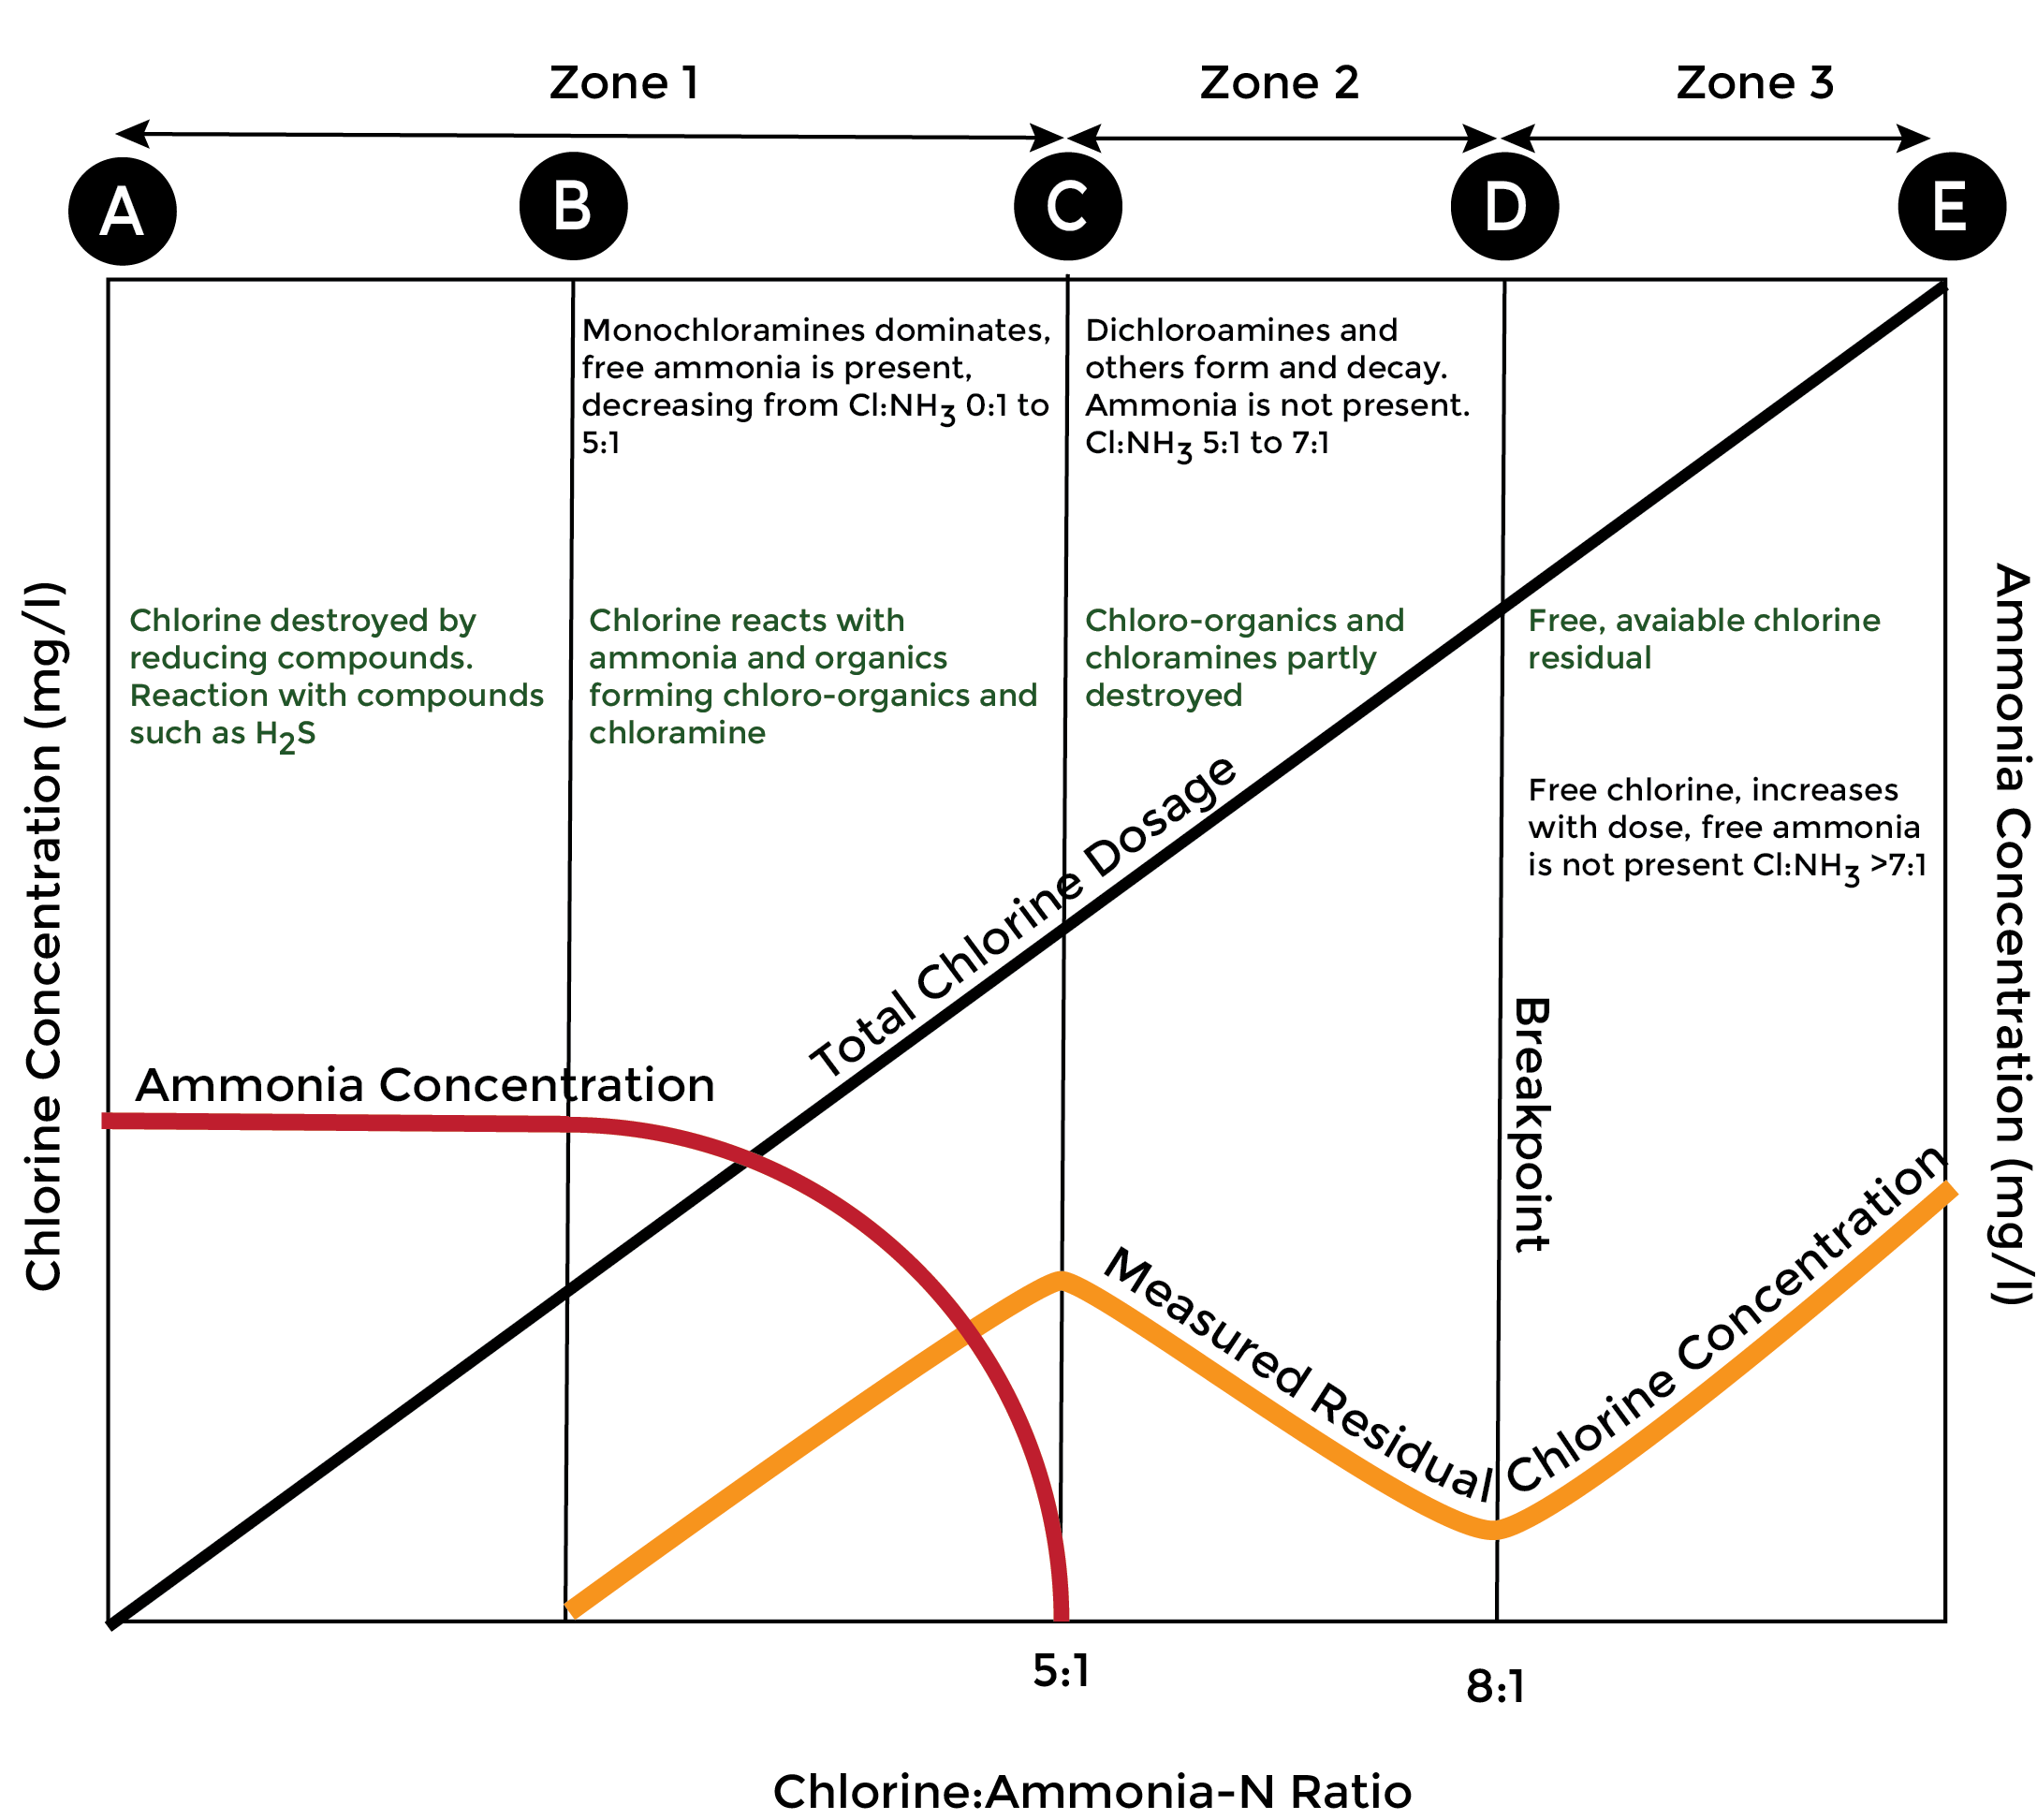
\includegraphics[scale=0.24]{BreakpointChlorination}
			\begin{itemize}
				\item Point A is at the beginning of chlorine application
				\item Between Points A and B, the chlorine dosage produces no residual because of an immediate chlorine demand caused by fast-reacting ions from metal salts and H$_2$S.
				\item Point B is the beginning of the reaction between chlorine and ammonia present
				\item Mono and dichloramines are formed between points B and C
				\item Zone 1 - between points A and C, is the combined zone and has mono and dichloramines and ammonia.  Monochloramines is a stable disinfectant while dichloramines is a strong disinfectant but unstable.
				\item After the maximum combined residual is reached (point C), further chlorine doses decrease the residual due to chloramine oxidation to dichloramine, occurring between points C and D.  This is Zone 2 - Breakpoint Zone
				\item Point D represents the breakpoint - the point at which chlorine demand has been satisfied and additional chlorine appears as free residuals
				\item Between points D and E, free available residual chlorine increases in direct proportion to the amount of chlorine applied.  This is Zone 3 which is the free chlorine zone and has hypochlorous acid but no ammonia.
								\item Breakpoint chlorination is the application of sufficient chlorine beyond the chlorine demand to maintain a free available chlorine residual.\\  Theoretically chlorine requirement = Wt. NH$_3$-N x 7.6\\
								In practice (Margin of safety)     = Wt. NH$_3$-N x 10\\
				\item After the breakpoint, free chlorine residuals develop. Free chlorine residuals usually destroy odors, kill microorganisms and oxidize organic matter.

			\end{itemize}
			\begin{itemize}
				\item Factors that affect breakpoint chlorination are initial ammonia nitrogen concentration, pH, temperature, and demand exerted by other inorganic and organic species
				\item Weight ratio of chlorine applied to initial ammonia nitrogen must be 8:1 or greater for the breakpoint to be reached. If the weight ratio is less than 8:1, there is insufficient chlorine present to oxidize the chlorinated nitrogen compounds initially formed
				\item When instantaneous chlorine residuals are required, the chlorine needed to provide free available chlorine residuals may be 20 or more times the quantity of ammonia present. Reaction rates are fastest at pH 7-8 and high temperatures
			\end{itemize}
\subsection{Chlorine dosing terms}\index{Chlorine dosing terms}
\begin{itemize}
\item \textbf{Chlorine dose} \index{Chlorine dosing terms!Chlorine dose} - the amount of chlorine added to the system. It can be determined by adding the desired residual for the finished water to the chlorine demand of the untreated water. Dosage can be either milligrams per liter (mg/L) or pounds per day (lb/day).

\item \textbf{Chlorine Demand} \index{Chlorine dosing terms!Chlorine demand}  - the amount of chlorine consumed by iron, manganese, turbidity, algae, and microorganisms in the water. Because the reaction between chlorine and microorganisms is not instantaneous, demand is relative to time. For instance, the demand 5 minutes after applying chlorine will be less than the demand after 20 minutes. 

\item \textbf{Free chlorine} \index{Chlorine dosing terms!Free chlorine}  - free chlorine refers to all chlorine present in the water as Cl$_2$(g), HOCl(aq) and OCl$^-$(aq).

\item \textbf{Combined residual} \index{Chlorine dosing terms!Combined residual} - is the result of combining free chlorine with nitrogen compounds. Combined residuals are also referred to as chloramines. 

\item \textbf{Total chlorine residual} \index{Chlorine dosing terms!Total chlorine residual} - is the mathematical combination of free chlorine and combined residuals. Total residual can be determined directly with standard chlorine residual test kits.  Residual, like demand, is based on time. The longer the time after dosage, the lower the residual will be, until all of the demand has been satisfied. Residual, like demand, is expressed in $\mathrm{mg} / \mathrm{L}$. The presence of a free residual usually provides a high degree of assurance that the disinfection of the water is complete. 

$$\mathrm{Chlorine Dose} (\mathrm{mg} / \mathrm{L})= \mathrm{Chlorine Demand}+ \mathrm{ Chlorine Residual}$$

\item Theoretically, while microorganisms are killed as the chlorine demand is being satisfied, disinfection is generally the result of chlorine residual or the amount of chlorine remaining after the chlorine demand has been satisfied.
\end{itemize}



\subsection{Contact Time}\index{Contact Time (CT)}
\begin{itemize}
\item Contact time is the amount of time which the chlorine has to react with the microorganisms in the water, which will equal the time between the moment when chlorine is added to the water and the moment when that water is used by the customer.
\item The longer the contact time, the more efficient the disinfection process is. When using chlorine for disinfection a minimum contact time of 30 minutes is required for adequate disinfection.
\item Contact time is just as important as the chlorine residual in determining the efficiency of chlorination.  
\item An operator measures the amount of contact time available at the plant before the water goes out to the public to ensure that $99.9 \%$ of giardia lamblia is either removed with filtration or inactivated with chlorine before the water gets to the public. 
\item The operator compares the contact time at the plant to the CT tables provided by the EPA.
\item As long as the contact time the operator measures at the plant is greater than that required by the EPA, the water passes the disinfection portion of the treatment process.

\item The "baffling efficiency" of a tank is used to determine chlorine contact time in the tank. If the water used to calculate disinfection contact time moves through a storage tank, pressure tank, or pipes too quickly, the situation is called "shortcircuiting". 
\item Some vessels provide better contact time than others do. Water systems can modify reservoirs to improve the baffling efficiency. 
\item In some cases little or no baffling efficiency can be awarded. Pipes with a length to width ratio of 150 or more typically have a baffling efficiency of 100 percent.
\item Table below provides theoretical baffling factors for various baffling conditions and factors.
\begin{table}[h!]
  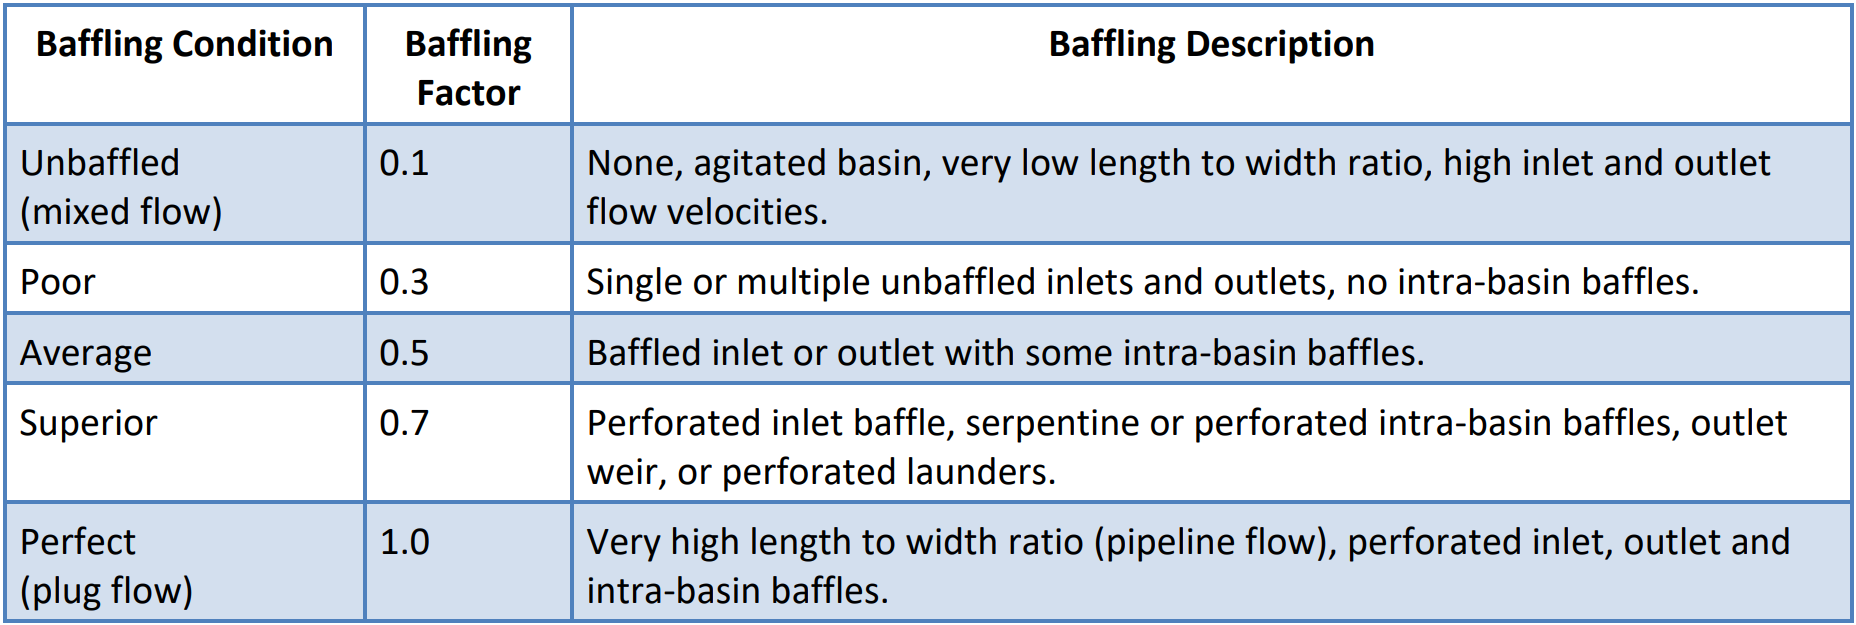
\includegraphics[width=\linewidth]{BafflingFactors}\index{baffling factors}
    \caption{Theoretical baffling factors}
\end{table}
\end{itemize}
In summary, to calculate CT you must know:

\begin{enumerate}
  \item The contact time (T) for each water system component between the chlorine injection point and where free chlorine is measured before the first customer.

  \item The volume and baffling efficiency of each component.

  \item The peak flow through each component.

  \item The free chlorine residual measured downstream of all the components and upstream of the first customer.

\end{enumerate}
When calculating Contact Time, use the lowest volume of water in the tank under non-emergency/normal operating conditions.

The following steps have been set up to help operators determine contact time.

Step 1: Determine the time available in the basin at peak flow. Multiply the basin volume by the baffling factor and divide by the Peak Hourly Flow to determine the Time portion of the contact time equation.
$$
\text { Time }(\min )=\frac{\text { Basin Volume }(\text { gal }) \mathrm{x} \text { baffling factor }}{\text { Peak Hourly Flow }(\mathrm{gpm})}
$$
Step 2: Determine the contact time available at peak flow. Multiply the Time by your chlorine concentration at peak hourly flow. This is the Contact Time you have available.

Available Contact Time $(\min \mathrm{mg} / \mathrm{L})=$ Time $(\mathrm{min}) \times$ Chlorine concentration $(\mathrm{mg} / \mathrm{L})$

Step 3: Find the required Contact Time (CT) from the tables at peak flow. Determine the CT required by the EPA. You need to do this by looking up the CT from the CT tables provided using your $\mathrm{pH}$, temperature and chlorine concentration.

Step 4: Does your water system meet CT requirements?

Compute the inactivation ratio by dividing the actual contact time by required contact time. If the rateo is greater than 1 , then your water system met its contact time requirements. If you cannot meet contact time, you can either increase your storage volume or increase your disinfectant residual.

Inactivation Ratio $=\dfrac{\text { Actual Contact Time }}{\text { Required Contact Time }}$

\textbf{Example:}
Your campground has a 5,000 gallon steel tank. An engineer has determined that the baffling factor for the tank is $0.3$. The flow of water through the system is determined to be 15 gallons per minute at maximum flow conditions. The pH is $7.0$ and the temperature is 10 Celsius. Determine whether or not your campground meets contact time requirements at $1.5 \mathrm{mg} / \mathrm{L}$ chlorine.

Step 1:
$$
\begin{aligned}
&\text { Time }(\min )=\frac{5,000 \mathrm{gal} \times 0.3}{15 \mathrm{gpm}} \\
&\text { Time }(\min )=100
\end{aligned}
$$
Step 2: Available Contact Time ( $\min \mathrm{mg} / \mathrm{L})=$ Time $(\mathrm{min}) \times$ Chlorine concentration $(\mathrm{mg} / \mathrm{L})$

Available Contact Time $(\min \mathrm{mg} / \mathrm{L})=100 \mathrm{~min} \times 1.5 \mathrm{mg} / \mathrm{L}$

Available Contact Time $(\min \mathrm{mg} / \mathrm{L})=150$

Step 3: Look up the contact time that you need to achieve from the applicable EPA CT Table - Chlorine disinfectant, pH=7.0, 1.5 mg/l chlorine residual and temperature=10$^o$C


\begin{table}[htp]
\begin{center}
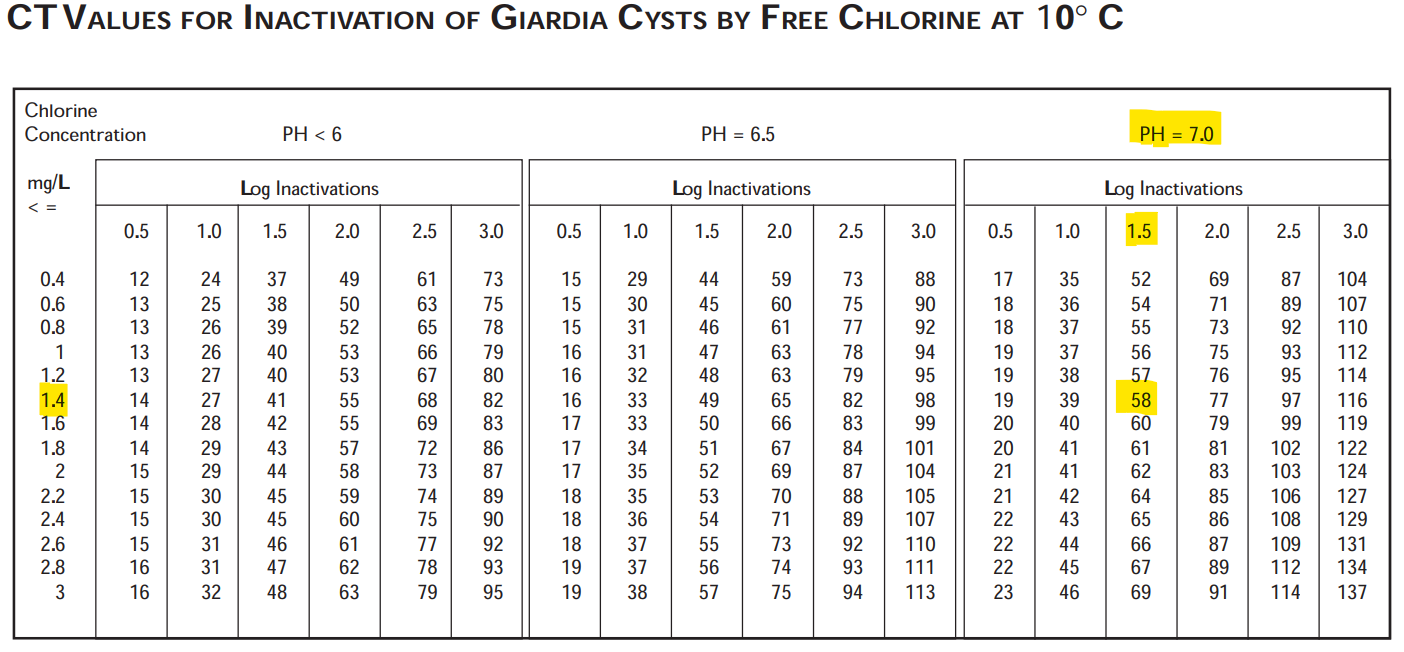
\includegraphics[width=\linewidth]{CTValueGiardia10C}\\
\captionof{table}{EPA - CT table }%\caption{}
\end{center}
\end{table}

You will notice under the Chlorine Concentration $(\mathrm{mg} / \mathrm{L})$ column, $1.5 \mathrm{mg} / \mathrm{L}$ is not listed, so use the next lowest chlorine residual, $1.4 \mathrm{mg} / \mathrm{L}$. Look at the table at $1.4 \mathrm{mg} / \mathrm{L}$ and go across to the $\mathrm{pH}=7.0$. The CT required for compliance, from the table, is 58 mg/l-min.

Step 4: Is the inactivation ratio greater than 1 ? Divide 150 by 58 to get 2.6. Since 2.6 is greater than 1 your system did meet the contact time requirements.
$$
\begin{aligned}
&\text { Inactivation Raio }=\frac{150}{58} \\
&\text { Inactivation Raio }=2.6
\end{aligned}
$$
\section{Chlorine dioxide}\index{Chlorine dioxide}
\begin{itemize}
\item Chlorine dioxide, a greenish-yellow gas, produced by reacting sodium chlorite with chlorine or an acid.
\item Because it is explosive under pressure and difficult to transport, it is generated on-site by reacting chlorite with chlorine or hydrochloric acid.  
\item Chlorine dioxide is a strong disinfectant.
\item The efficiency is pH dependent; is is optimum at a pH of 3 to 5.  
\end{itemize}

\subsection{Advantages of chlorine dioxide}\index{Chlorine dioxide!Advantages}
\begin{itemize}
\item Chlorine dioxide has a higher oxidation capacity than most species of chlorine. 
\item It does not hydrolyze to form an acid, and therefore is less corrosive.
\item Unlike chlorine, it acts only by oxidation and does not combine with organic compounds to form environmentally hazardous disinfection by-products.
\item Its effectiveness is not affected by ammonia and pH, and does not produce THMs.
\item Its effectiveness against Giardia and Cryptosporidium is reported as better than chlorine.
\end{itemize}

\subsection{Disdvantages of chlorine dioxide}\index{Chlorine dioxide!Disadvantages}
\begin{itemize}
\item Chlorine dioxide is unstable and reverts to chlorite and therefore it needs to be generated at the site and applied immediately.
\item It is relatively expensive to generate
\item It is explosive at a concentration above 10 percent in the air.
\item It forms chlorites and chlorates which cause an anemic condition in some individuals.
\end{itemize}

\section{Ultraviolet (UV) disinfection}\index{Ultraviolet (UV) disinfection}

\begin{itemize}
	\item UV Disinfection of wastewater is conducted in specially designed reactors fitted with ultraviolet lamps producing energy in the UV-C range (200-400 nm)
	\item The UV lamps produce light photons that attack the microorganisms in wastewater as it flows through the reactor. 
	\item Within only a few seconds of exposure to the UV energy, the DNA of the microorganisms is permanently altered and the bacteria can no longer reproduce or infect those coming in contact with the water. 
	\item UV for wastewater disinfection has been in use for more than 50 years
	\item Increased interest after the discovery in the late 1990's of its remarkable effectiveness against Cryptosporidium parvum and Giardia lamblia - pathogens in surface waters which can find its way into the drinking water supplies
	\item The big advantage of UV disinfection over chlorine and ozone is that UV does not involve chemical use.
	\item The UV dose expressed as $\frac{mJ-sec}{cm^2}$ or $\frac{\mu W-sec}{cm^2}$ is the product of UV intensity (energy per unit surface area) - mJ/$cm^2$ or $\mu$W/$cm^2$ and residence time - sec.  

\end{itemize}

\subsection{Advantages of UV disinfection}\index{Ultraviolet (UV) disinfection!Advantages}
	\begin{itemize}
		\item Very effective against bacteria, fungi, protozoa
		\item Independent on pH, temperature, and other materials in water
		\item Smaller reactor size requirement compared to chlorination
	\end{itemize}
\subsection{Disadvantages of UV disinfection}\index{Ultraviolet (UV) disinfection!Disadvantages}
\begin{itemize}
	\item Suspended solids, slime growth, turbidity, and color present in wastewater will inhibit the effectiveness of UV
	\item No lasting residuals
	\item UV light tends to ionize compounds and break them apart (i.e. nitrate could become nitrite in UV light), causing toxic effects on the effluent.
	\item Expensive
\end{itemize}

\section{Ozonation}\index{Ozonation}
		\begin{itemize}
			\item Ozone ($O_3$) is the triatomic form of oxygen - it is composed of three oxygen atoms.
			\item Under normal conditions ozone is unstable and quickly decomposes to the more stable gaseous oxygen, $O_2$. 
			\item Because of its instability, ozone cannot be stored and thus generated at the point of application. 
			\item Ozone is generated by passing air or oxygen through an electrical discharge - the noticeable clean smell in the air after a thunder and lightning storm is likely due to the formation of ozone due to the lightning bolts passing through the atmosphere.
			\item Ozone is thirteen times more soluble in water than oxygen. 
			\item Ozone is even more effective against some viruses and cysts than chlorine.
			\item It has the added advantage of leaving no taste or odor and is unaffected by pH or the ammonia content of the water. 
			\item When ozone reacts with reduced inorganic compounds and with organic material, an oxygen atom instead of a chloride atom is added to the organics, the end result being an environmentally acceptable compound.
			\item Ozone disinfects 3,100 times faster than chlorine. It has also been found that disinfection occurs within contact times of 3 to 8 seconds.
			\item Viricidal properties of ozone is exhibited at longer contact time of about 5 minutes needed.
			\item Any residual ozone in the effluent of the contactor disappears in a matter of seconds outside the contactor.
		\end{itemize}

\subsection{Advantages of ozonation}\index{Ozonation!Advantages}
	The advantages of ozonation include :
		\begin{itemize}
			\item Reduces colors, phenolics, cyanides, oxygen demanding matter, turbidity and surfactants
			\item Increases dissolved oxygen
			\item Does not produce any significant toxic by-products
			\item Increases suspended solids reduction
		\end{itemize}

\subsection{Disadvantages of ozonation}\index{Ozonation!Disadvantages}
	The disadvantages of ozonation include :
		\begin{itemize}
			\item High capital cost
			\item High electric consumption
			\item Highly corrosive, especially with steel or iron and even oxidizes Neoprene
			\item Ozone promotes formation of bromates and brominated DBPs.
		\end{itemize}

\section{Summary of disinfectants' attributes}\index{Disinfectants' attributes}
\begin{itemize}
\item [\ding{252}] Pathogen Destruction: Ozone > ClO$_2$ > Chlorine >> Chloramines
\item [\ding{252}] Residual Stability: Chloramines > Chlorine > > ClO$_2$ > Ozone
\item [\ding{252}] Other Treatment Benefits: Chlorine > Ozone, \& ClO$_2$ >>  Chloramines
\item [\ding{252}] Disinfection By-Product Yield: Chloramines >> ClO$_2$ Ozone \& Chlorine
\end{itemize}

